
\begin{minipage}{0.5\linewidth}
    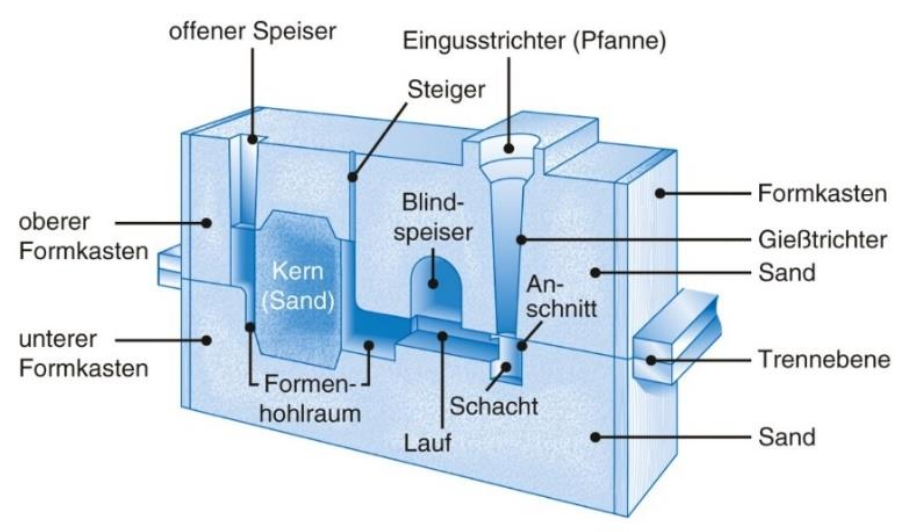
\includegraphics[width = 40mm]{src/images/Giesssystem.png}
\end{minipage}
    \begin{minipage}{0.5\linewidth}
        \begin{itemize}
            \item Anschnitt: System der Zuleitungen.
            Dient zur Steuerung von Füll- und Erstarrungs-
            vorgang, sowie zum Auffangen von Verunreini-
            gungen.
            \item Speiser: Reservebehälter für Schmelze, die in
            die Hohlräume nachfliesst, um Schwindung
            auszugleichen. \\
            Verhältnis von Volumen zu Ober-
            fläche sollte grösser sein als beim Gussstück.
        \end{itemize}
    \end{minipage}
    \vspace{1mm}
